% !TEX TS-program = pdflatex
% !TEX encoding = UTF-8 Unicode

%\documentclass[12pt,a4paper]{memoir} % for a long document
\documentclass[12pt,a4paper,article]{memoir} % for a short document

\usepackage[utf8]{inputenc} % set input encoding to utf8

%%% PAGE DIMENSIONS
% Set up the paper to be as close as possible to both A4 & letter:
\settrimmedsize{11in}{210mm}{*} % letter = 11in tall; a4 = 210mm wide
\setlength{\trimtop}{0pt}
\setlength{\trimedge}{\stockwidth}
\addtolength{\trimedge}{-\paperwidth}
\settypeblocksize{*}{\lxvchars}{1.618} % we want to the text block to have golden proportionals
\setulmargins{50pt}{*}{*} % 50pt upper margins
\setlrmargins{*}{*}{1.618} % golden ratio again for left/right margins
\setheaderspaces{*}{*}{1.618}
\checkandfixthelayout 
\usepackage{enumitem}
\setitemize{noitemsep,topsep=0pt,parsep=0pt,partopsep=0pt}
\usepackage{xcolor,listings}
\usepackage{textcomp}
\lstset{upquote=true}
\usepackage{graphicx}
\usepackage{hyperref}
\hypersetup{
  colorlinks=true,
  linkcolor=blue,
  urlcolor=blue
}

%%% \maketitle CUSTOMISATION
% For more than trivial changes, you may as well do it yourself in a titlepage environment
\pretitle{\begin{center}\sffamily\huge\MakeUppercase}
\posttitle{\par\end{center}\vskip 0.5em}

%%% ToC (table of contents) APPEARANCE
\maxtocdepth{subsection} % include subsections
\renewcommand{\cftchapterpagefont}{}
\renewcommand{\cftchapterfont}{}     % no bold!

%%% HEADERS & FOOTERS
\pagestyle{ruled} % try also: empty , plain , headings , ruled , Ruled , companion

%%% CHAPTERS
\chapterstyle{hangnum} % try also: default , section , hangnum , companion , article, demo

\renewcommand{\chaptitlefont}{\Huge\sffamily\raggedright} % set sans serif chapter title font
\renewcommand{\chapnumfont}{\Huge\sffamily\raggedright} % set sans serif chapter number font

%%% SECTIONS
\hangsecnum % hang the section numbers into the margin to match \chapterstyle{hangnum}
\maxsecnumdepth{subsection} % number subsections

\setsecheadstyle{\Large\sffamily\raggedright} % set sans serif section font
\setsubsecheadstyle{\large\sffamily\raggedright} % set sans serif subsection font

\newlength\drop
\makeatletter
\newcommand*\titleM{\begingroup%
\setlength\drop{0.08\textheight}
\centering
\vspace*{\drop}
{\Huge\bfseries Technical Interview}\\[\baselineskip]
%{\scshape MAN-AHL}\\[\baselineskip]
\vfill

\includegraphics[width=0.6\textwidth]{img/logo.png}\par\vspace{1cm}
\vfill
{\Huge\scshape Fadil Mokhchane \\ 
\small \href{https://www.linkedin.com/in/fadil/}{LinkedIn} }\par
\vspace{1cm}

\includegraphics[width=0.2\textwidth]{img/harrington.jpg}\par
\vfill
{\scshape \@date}\par
\vspace*{2\drop}
{\scshape \small Version 0.1}\par
\endgroup}
\makeatother
%% END Memoir customization

\title{Technical Interview}
\author{Fadil Mokhchane}
%\date{ August 2017} % Delete this line to display the current date
%%% BEGIN DOCUMENT
\begin{document}


\begin{titlingpage}
\titleM
\end{titlingpage}

\newpage
\tableofcontents* % the asterisk means that the contents itself isn't put into the ToC
%\clearpage %or \cleardoublepage
\phantomsection
\listoffigures
%\listoftables
\newpage

%-------------------------------------------------------------------------------
\chapter{Algorithm}
\section{Question}
Implement the method nextNum() and a minimal but effective set of unit tests. 
Implement in the language of your choice, Python is preferred, but Java and 
other languages are completely fine. 
Make sure your code is exemplary, as if it was going to be shipped as part of a production system.

As a quick check, given Random Numbers are $[-1, 0, 1, 2, 3]$ and 
Probabilities are $[0.01, 0.3, 0.58, 0.1, 0.01]$ if we call nextNum() 100 times 
we may get the following results. As the results are random, these particular results are unlikely.
\begin{itemize}
	\item -1: 1 times 
	\item 0: 22 times
	\item 1: 57 times 
	\item 2: 20 times
	\item 3: 0 times 
\end{itemize}

\section{The Problem}
We interpret the question as the following the mathematical problem. 
We define a $X$ as a discrete random variable. 
As input, we have a $k$ values, $x_i$, with their associated probabilities, $P_i$.

A discrete probability density function is a probability distribution charaterised 
by a probability mass function :
\[
	\forall i \in \left[1 ...  k\right], P\left[ X = x_i \right] = P_i  
\]
With
\[ 
	\sum_{i = 1}^k  P\left[ X = x_i \right]  = 1
\]
This probability mass function can be illustrated \autoref{fig:distribution} :
\begin{figure}[h!]
\begin{center}

\includegraphics[width=0.5\textwidth]{img/distribution.png}
\caption{Probability Mass Function}
\label{fig:distribution}
\end{center}
\end{figure}

We would like to build a generator that picks $x_i$ given their probabilities
$P_i$. 
In order to make sure we generate $x_i$ with repesct to their original probabilities, 
we need to add a no $x_i$ selected if the sum of the $x_i$ is less than $1$.

This way we can build a discrete cumulative function for $X$, $F_x$, such as :
\begin{equation}
	F_x = P\left( X \leq x \right)
	\label{eq:cdf}
\end{equation}
Which can be illustrated with \autoref{fig:cdf2} :
\begin{figure}[h!]
\begin{center}
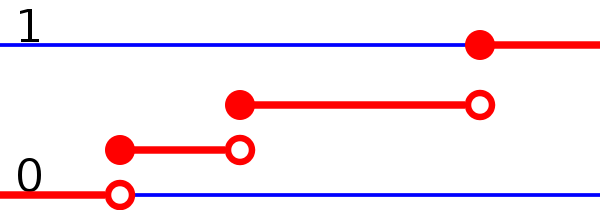
\includegraphics[width=0.5\textwidth]{img/cdf.png}
\caption{Discrete Cumulative Distribution Function}
\label{fig:cdf2}
\end{center}
\end{figure}

We then use a normal distribution to generate a number between $0$ and $1$.
\[
	f_x = \frac{1}{\sqrt{2 \pi}} e^{\frac{x^2}{2}}
\]
Using our discrete cumulative function, in \autoref{eq:cdf}, we can pick an $x_i$.
The probability density of the normal distribution with mean $0$ and variance $1$ is:

\section{Solution Proposed}
\subsection{Overview}

The key requirement is to deliver a production quality software.
This means that the code has to be well designed, efficient, portable and well tested.

The key features we would like to implement are:
\begin{itemize}
	\item Implement the generator,
	\item Create an User Interface, via Command Line Input,
	\item Compare various pseudo random number generator,
	\item Target $100\%$ testing coverage.
	\item Document the work.
\end{itemize}

\subsection{Design}
Hence we target the following archictecture, c.f. \autoref{fig:architecture1}.
\begin{figure}[h!]
\begin{center}
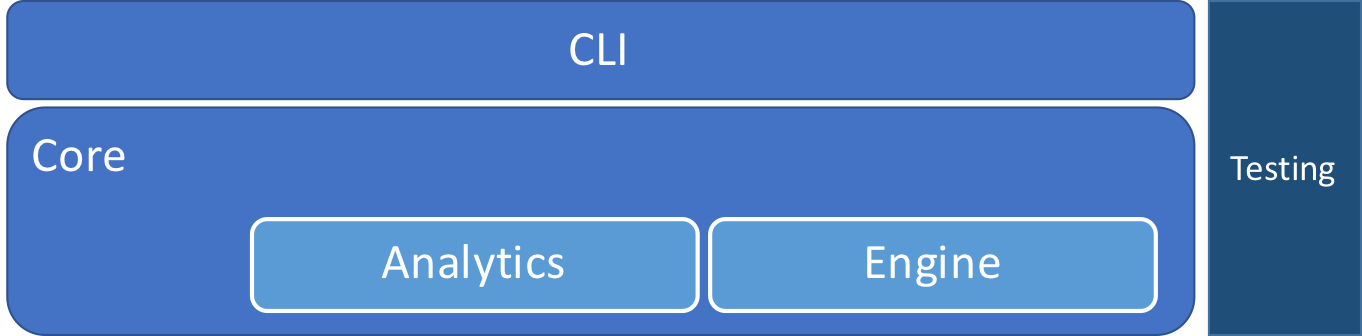
\includegraphics[width=0.8\textwidth]{img/architecture1.png}
\caption{Algorithm App Architecture}
\label{fig:architecture1}
\end{center}
\end{figure}
The various modules implement all the functionalities we need.
\begin{description}
	\item[Analytics] The mathematical functions required,
	\item[Engine] 	The various random numbers generator,
	\item[CLI] 		The command line input module,
	\item[Testing] 	The testing module. 
\end{description}

\subsection{Testing}
We need to test each module independtly, i.e. unit testing, and when they 
are all used together, i.e. integration testing.

Due to our limited testing environment, c.f. \autoref{apx:testing.env},
we limit ourselves to the following tests.

\emph{TBC}

\subsection{UI}
The UI is command line input allowing the user to run each feature.

%-------------------------------------------------------------------------------
\newpage
\chapter{SQL}
\section{Question}
Given the following tables
\begin{lstlisting}[
           language=SQL,
           showspaces=false,
           basicstyle=\ttfamily,
           numbers=left,
           numberstyle=\tiny,
           commentstyle=\color{gray}
        ]
CREATE TABLE Product
(
product_id number primary key,
name varchar2(128 byte) not null,
rrp number not null,
available_from date not null
);
CREATE TABLE Orders
(
order_id number primary key,
product_id number not null,
quantity number not null,
order_price number not null,
dispatch_date date not null,
foreign key (product_id) references Product(product_id)
);
\end{lstlisting}
Write an sql query to find books that have sold fewer than 10 copies in the last year, 
excluding books that have been available for less than 1 month.

Some example data, intended to give an idea of the sort of data that might exist, 
can be found below. Note that the data is not complete, 
nor does it necessarily cover all the cases that might be encountered.

\begin{center}
    \begin{tabular}{| l | l | l | l |}
    \hline
	product\_id & name & rrp & available\_from \\
	\hline 
	101 & Bayesian Methods for ...& 94.95 & (last thursday) \\
	102 & (next year) in Review (preorder) & 21.95 & (next year) \\
	103 & Learn Python in Ten Minutes & 2.15 & (three months ago) \\
	104 & sports almanac (1999-2049) & 3.38 & (2 years ago) \\
	105 & finance for dummies & 84.99 & (1 year ago)  \\
	\hline
    \end{tabular}
\end{center}
\begin{center}
    \begin{tabular}{| l | l | l | l | l |}
    \hline
	order\_id & product\_id & quantity & order\_price & dispatch\_date \\
	\hline 
	1000 & 101 & 1 & 90.00 & (two months ago) \\
	1001 & 103 & 1 & 1.15 & (40 days ago) \\
	1002 & 101 & 10 & 90.00 & (11 months ago) \\
	1003 & 104 & 11 & 3.38 & (6 months ago) \\
	1004 & 105 & 11 & 501.33 & (two years ago) \\
	\hline
    \end{tabular}
\end{center}

\section{Solution Proposed}
We can solve the problem by running a query like:
\begin{lstlisting}[
           language=SQL,
           showspaces=false,
           basicstyle=\ttfamily,
           numbers=left,
           numberstyle=\tiny,
           commentstyle=\color{gray}
        ]
SELECT p.name
FROM  (
   SELECT product_id, name FROM product 
      WHERE available_from >=  (today - 1 month)
) p
INNER JOIN (
   SELECT product_id, SUM(quantity) nb FROM orders
      GROUP BY product_id
      WHERE dispatch_date <= (today - 1 year)
) o
   ON p.product_id = o.product_id
WHERE 
   o.nb < 10
\end{lstlisting}

The key issue here in order to produce a production-like quality is 
to test the query proposed.

\subsection{Overview}
We will extend our App by adding a database layer to create and query 
the tables.
We extend also our testing layer to create datasets in order to test
the accuracy and efficiency of our query.

\subsection{Design}
Hence we target the following archictecture, c.f. \autoref{fig:architecture2}.
\begin{figure}[h!]
\begin{center}
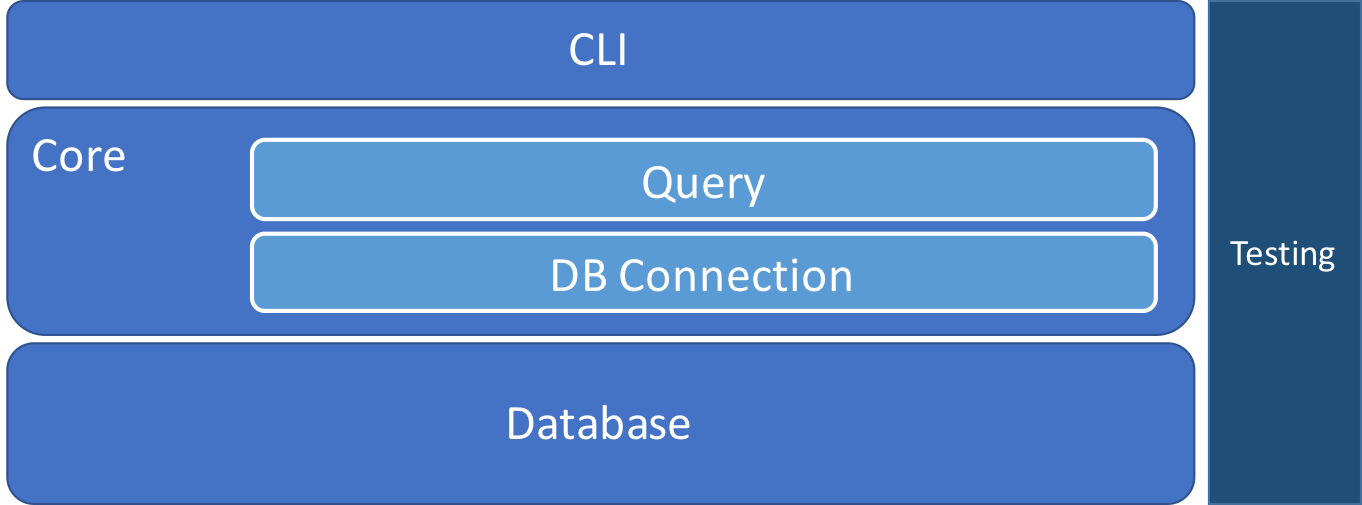
\includegraphics[width=0.8\textwidth]{img/architecture2.png}
\caption{SQL App Architecture}
\label{fig:architecture2}
\end{center}
\end{figure}

\subsection{Testing}
We unfortunately lack the production tools to analyse the query execution.
Without the access to the query plan of execution, we can only on our
experience and empirical tests to create the best query possible.

Therefore we have simple datasets to test the limiting cases and 
large datasets to test the performance of our query.

We have access to a limited hardware, c.f. \autoref{apx:testing.env}, 
therefore the performance are slow.

\subsection{UI}
We extend the CLI to include the following command :
\begin{description}
	\item[TBC] ...
\end{description}

%-------------------------------------------------------------------------------
\newpage
\chapter{Discussion}
\section{Implementation}
In order to understand and share the creation process, 
we share the Git log in \autoref{apx:git.log}. 
Having a git log allows also rolling back changes, if needed.

We tried to follow a Test Driven Development process as 
demonstrated by the Git log.

\section{Testing}
The testing environment is described in \autoref{apx:testing.env}.

\section{Extension}
Here is a list of possible extension we could add.
\begin{description}
	\item [Testing]
	Add some qualitative testing, by displaying the distribution generated 
	by the random number generators.
	
	Run the tests on different environments to ensure the portability of 
	the code.
	\item [UI] 
	A nice extension would be to add a Graphic User Interface,
	using the library 
	\href{https://hackage.haskell.org/package/threepenny-gui}{threepenny-gui}
	to create a portable Web application.
	
	Also we could integrate a plot library to display the distribution of 
	random numbers.
	\item[Database]
	We could add features to store and retrieve the results.
	\item[Continuous Integration]
	The fact that we tested only Mac OS, c.f. \autoref{apx:testing.env} is 
	not production like.
	We would like to run on various environment, a simple extension would 
	be to run on Travis and AppVeyor website accessible via GitHub.
\end{description}

%-------------------------------------------------------------------------------
\newpage
\appendix
\addcontentsline{toc}{chapter}{Appendices}
\chapter{Installation} \label{apx:installation}

Here are the steps to install the App.
\begin{enumerate}
	\item Download Haskell via this \href{https://www.haskell.org/platform/}{link}.
	\item Install following the instructions given by the installer.
	\item Use cabal to download the require packages :
\begin{lstlisting}[
           language=SQL,
           showspaces=false,
           basicstyle=\ttfamily,
           numbers=left,
           numberstyle=\tiny,
           commentstyle=\color{gray}
        ]
	cabal install TBC
\end{lstlisting}
\end{enumerate}

%-------------------------------------------------------------------------------
\newpage
\chapter{Testing Environment} \label{apx:testing.env}

Given that I don't have access to my server this week, 
we run the test on a MacBook Pro 2008 4GB DDR3 Intel Core Duo 2.53GHz.
It has 250GB harddisk, not SSD. 

We are using Haskell version 8.2.1 on MacOS.

%-------------------------------------------------------------------------------
\newpage
\chapter{Haskell Libraries} \label{apx:haskell.libraries}

%-------------------------------------------------------------------------------
\newpage
\chapter{Git Log} \label{apx:git.log}
We provide below the git log, as we are simulating a production environment.

%-------------------------------------------------------------------------------
\newpage
\chapter{Code} \label{apx:code}
We provide below the code.

\end{document}
